% !TEX root = ../../report.tex

\section{The SoBazar Data}
    This sections is dedicated to exploring the data set to be worked with.
    This includes how the data was preprocessed before utilizing it, the summary of the dataset, statistics and graphs about the data and findings from the data.

\subsection{Data Cleaning}
    \marginpar{Some better way of saying this; Data Preprocessing, Data Prefiltering, something}
    The data from soBazar came as is from the soBazar database, with the exception that the data had been anonymised, for privacy reasons.
    It contained therefore some unnecessary events.
    The data was therefore cleaned by removing events containing test environment flags such as: test environment and applications run from simulator.
    What was left after the cleaning data was mainly events triggered by the users, and no created during applications testing.

\subsection{Dataset Summary}
    The data from soBazar is so call implicit~\ref{sec:implicit} and is based on the different set of events triggered by the users of the soBazar application.

\subsubsection{Event Metadata}
    When an event is triggered a set of information is stored regarding the event.
    This data is used to make recommendations for the users though converting the implicit feedback to implicit ratings.

    \begin{table}[H]
        \centering
        \begin{tabular}{l|l}
            \toprule
            \emph{Variable}     & \emph{Explanation}   \\ \hline
            "price"             & The price of the item which triggered the event \\ \hline
            "product\_id"       & The id of the item which triggered the event \\ \hline
            "storefront\_id"    & The store id from which the item originated \\ \hline
            "event\_id"         & What kind of event was triggered~\tablefootnote{Complete list of the different types of events can be found in table~\ref{table:events}} \\ \hline
            "event\_location"   & The location of the user when the event was triggered \\ \hline
            "ts"                & Unix timestamp in milliseconds of when the event was triggered \\ \hline
            "session"           & Which session number the event belongs too~\tablefootnote{This value is added at a later time. For two events to end up in the same session, the event has to be triggered within a certain period of time, and both be after the same application started-flag} \\ \hline
            "user\_id"          & The unique id of the user who triggered the event \\
            \bottomrule
        \caption[Event Metadata]{Table of some of the metadata collected from an event. The complete list can be found in table~\ref{table:completeEventData}}
        \label{table:eventData}
        \end{tabular}
    \end{table}

    %How much preference data?
    %Which events are interesting to look at?
% \subsubsection{Numbers}
    \begin{table}[H]
        \centering
        \begin{tabular}{l|l}
            \toprule
            \emph{What}        & \emph{Count}   \\ \hline
            Unique users ids   & 1235           \\ \hline
            Unique item ids    & 3386           \\ \hline
            Unique brands      & 16             \\ \hline
            Purchases          & 1484           \\ \hline
            Wants              & 7726           \\ \hline
            Item Clicks        & 14036          \\
            \bottomrule
        \caption[Dataset summary]{Table of the basic numbers regarding the soBazar dataset}
        \label{table:datasetSummary}
        \end{tabular}
    \end{table}
    \marginpar{input the updated data when/if we get a new dump from soBazar}

    % \begin{table}[H]
    %     \centering
    %     \begin{tabular}{l|l|l}
    %         Offer database length           & 7854   & ~ \\ \hline
    %         Event items length              & 4042   & ~ \\ \hline
    %         NonMatching values:             & 620    & ~ \\ \hline
    %         Items from Events not in Offer  & 7.89 \% & ~ \\
    %     \end{tabular}
    %     \caption[]{Items in events not in the actual offer database }
    % \end{table}

% \subsubsection{The Expected}
%     Event "app\_started", all have user\_id's
%     Event "app\_first\_started", all user\_id's are NULL
%     Event "user\_logged\_in", all have user\_id's... (assigned with login, event saved after login?)

% \subsubsection{The Strange}
%     NULL valued  for user\_id events: (Not all strange, but put together for readability)
%     facebook\_share\_changed

%     collection\_viewed  ignoring collection view-event as of now since the user\_id
%     is null. Could be valuable to use, though (30 000 events ignored) ...
%     potential workaround:
%         for each session do:
%             Filter all events on:
%                 session-ts-start to session-ts-end,
%                 allow: user\_id session-user-id and NULL
%                 Ip of user-session and ip of collection\_viewed
%                 storefront\_id's from session
%                     Populate collection\_viewed-user-id with session-user-id

%     Potential faulty user-id setting for ip-switch during a session, but expect few
%     occurrences of this

%     wantlist\_menu\_entry\_clicked
%     app\_became\_active

%     app\_first\_started
%     facebook\_login\_failed

%     > db.prod.distinct('event\_json.ipAddress').length
%     9033
%     > db.prod.distinct('event\_json.eventData.device\_id').length
%     2644
%     > db.prod.distinct('user\_id').length
%     1660

%     More devices than users, can't fill the blanks with device\_id

%     Q's:
%         app\_became\_active id's for better sessions?
%         store\_clicked vs. storefront\_clicked (23 vs. 19744)
%         API item-id's mapping to event product\_id's; how to map?


%     soBazar want to build a proper model.  Give input on how to build this model.
%     The supplier should know that an item is a jacket for instance.  Have something
%     to show on the 20. Should be better than what is already implemented.


\subsection{Graphs}
    Price ranges of all items (groupings)

    \begin{figure}[H]
        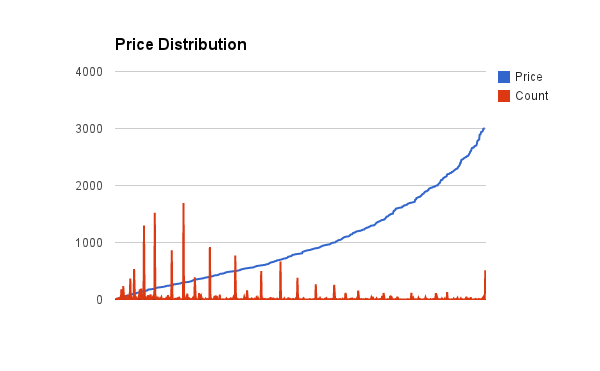
\includegraphics[width=5in]{image/price_distr.png}
        \centering
        \caption[Price distribution of items]{Here we see how them items are distributed on amount of items and price. The red bars indicates the amount of items with the belonging price (the blue line).
        All items priced over 3 000 are put in the same bucket, and is the reason for the last spike.
        We can see from this graph that the majority of the items are priced under 1 000 NOK}
        \label{figure:ratingdistr}
    \end{figure}

            (Distinct event locations)TODO

            Item time on market TODO maybe not that interesting alone


        complex 2.Deg:

            Count for different events

    \begin{figure}[H]
        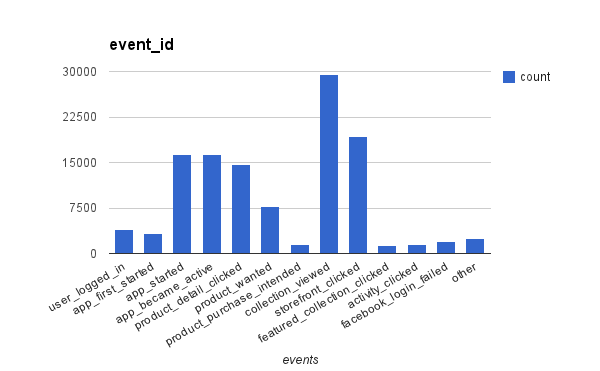
\includegraphics[width=5in]{image/event_id.png}
        \centering
        \caption[Count for different events]{some awesome text}
    \end{figure}

            Distinct events done on stores (shady)

    \begin{figure}[H]
        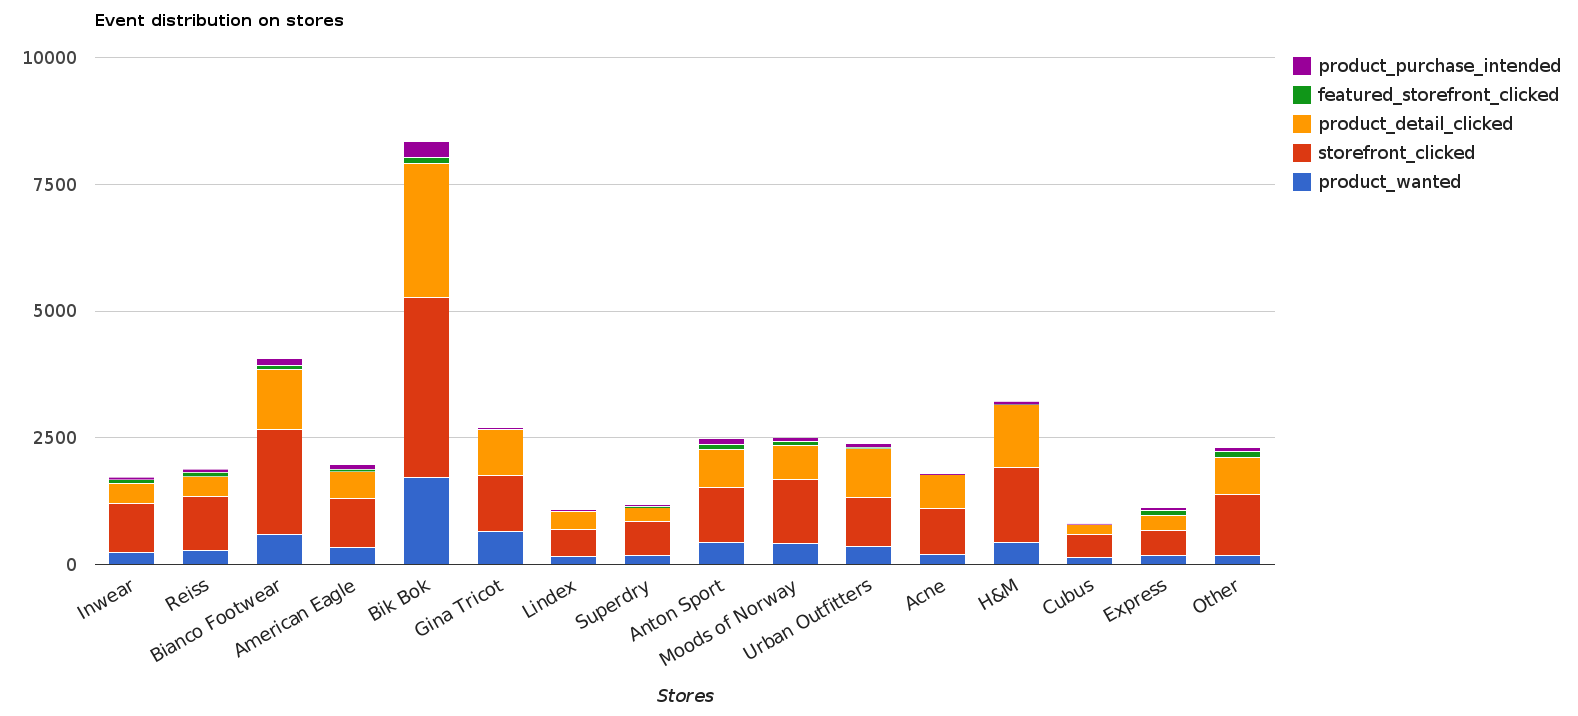
\includegraphics[width=5in]{image/event_distr.png}
        \centering
        \caption[Distribution of events on storefronts]{some awesome text}
    \end{figure}

    \begin{figure}[H]
        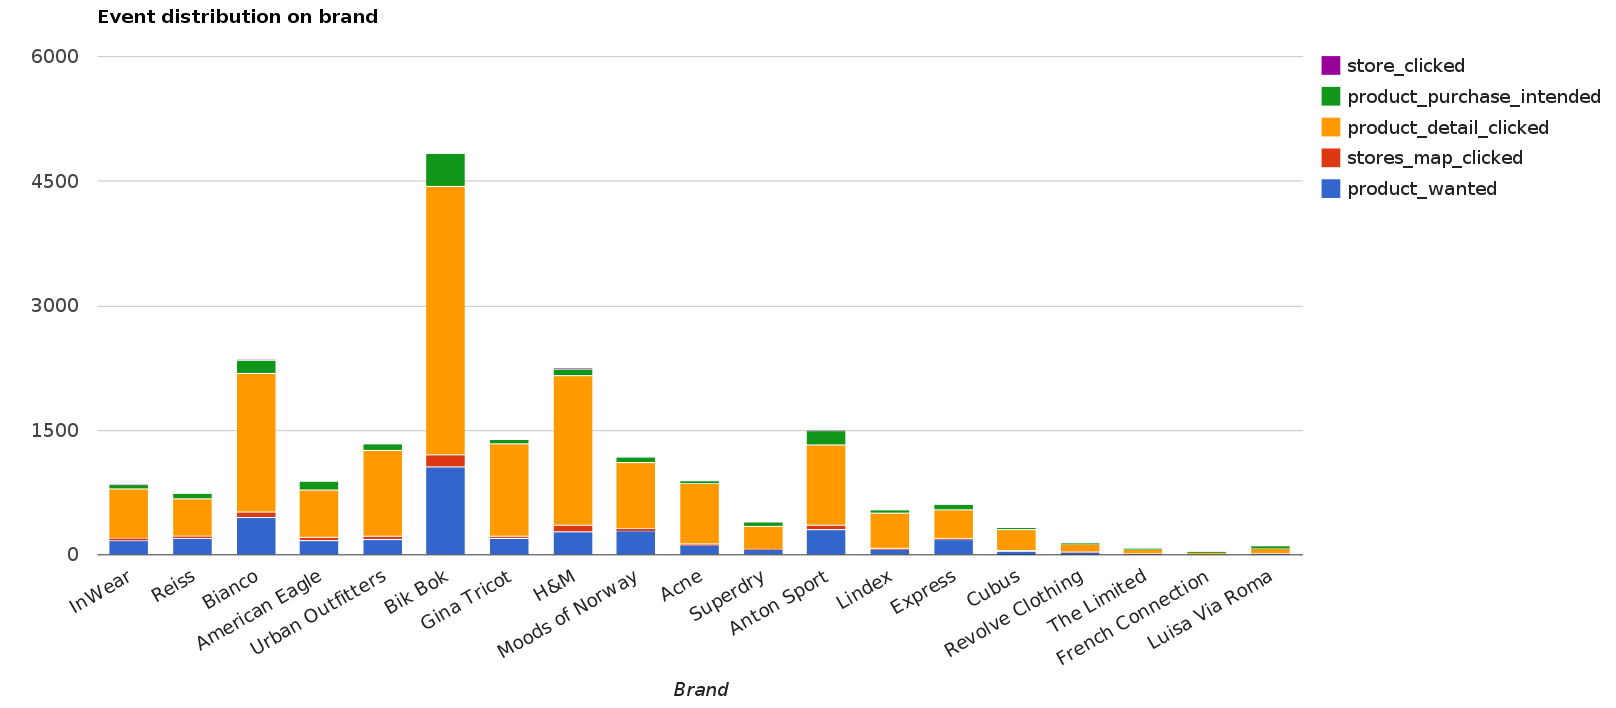
\includegraphics[width=5in]{image/brand_distr.png}
        \centering
        \caption[Distribution of events on brands]{some awesome text}
    \end{figure}

            peak online (slope-style) (events per day)

    \begin{figure}[H]
        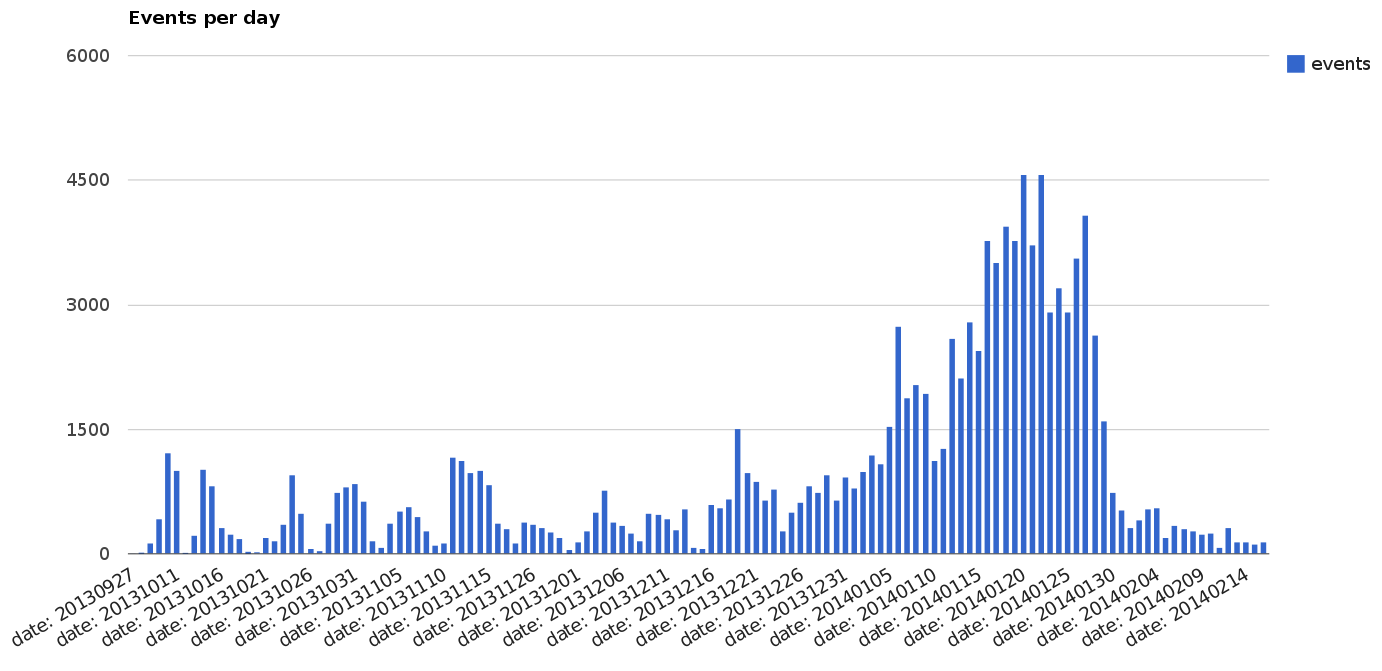
\includegraphics[width=5in]{image/events_per_day.png}
        \centering
        \caption[Distribution of events per day]{TODOsome awesome text}
    \end{figure}


            Price range of items in stores



            count User eventes
            user-item (how many items has a user "interacted" with)
            Count of unique items in item db also in event db
            Usable events regarding userid (events types with not null userid)
            (Plotting locations)

    \begin{figure}[H]
        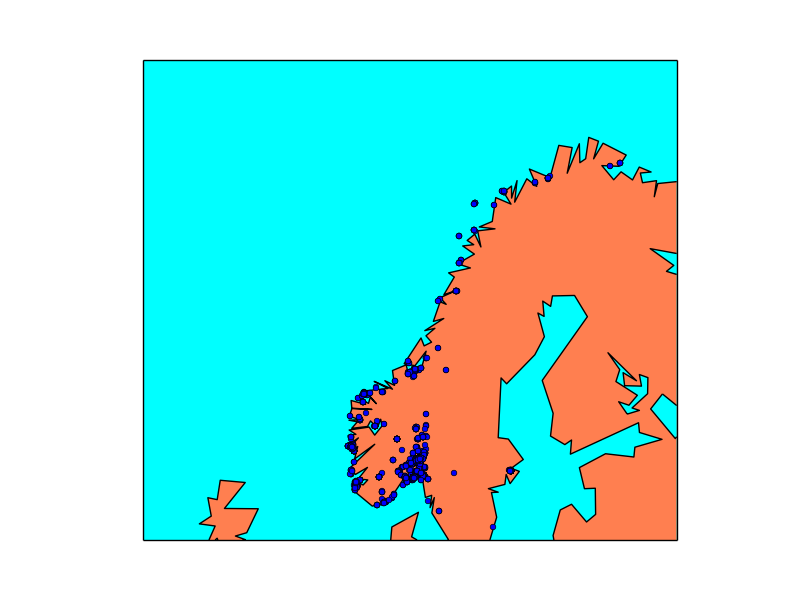
\includegraphics[width=5in]{image/simpleGeoPlot.png}
        \centering
        \caption[Simple plotting of event location]{TODOsome awesome text}
    \end{figure}


            unique Stores count for users

        complex 3.Deg:

            count Sessions for users (aprox: sessioncount)TODO

    \begin{figure}[H]
        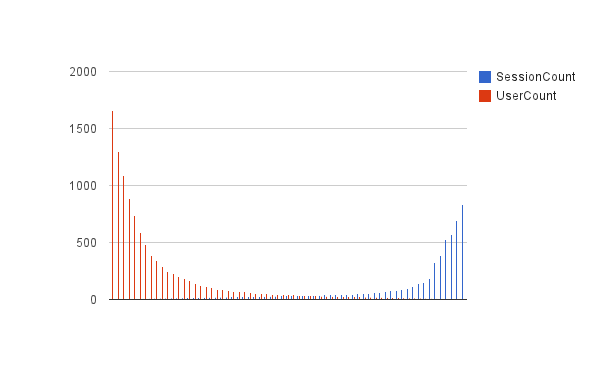
\includegraphics[width=5in]{image/global_sessioncount.png}
        \centering
        \caption[Count of sessions per user mapped with count of user with give
        session amount]{TODOsome awesome text}
    \end{figure}

            price span for user

        complex 4.Deg:

            Stats for sessions:

                Timespann of sessions for users (avg, max, min)
                Events per session (avg, max, min)
                Item viewtime for user in session
                Stores visited per session
                revisit time of items for user
                relationship with view, want and purchase
                time of session over lifetime of app
                user preferred price in session

        complex 5.Deg:

            Stats for global session stats:

                price vs view, want and purchase
                avg viewtime for an item (i know)
                Similarity of user favorite store, items viewed and items wanted?
                time of session over lifetime of app for all users (slope-style)

        complex 6.Deg:

        new:
            item timespan (first item interest - last item interest)

    \begin{figure}[H]
        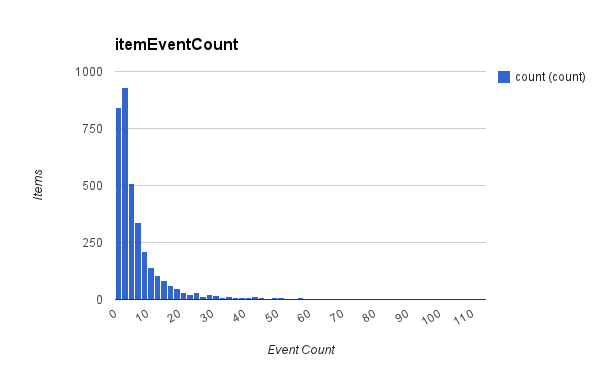
\includegraphics[width=5in]{image/item-event-count.png}
        \centering
        \caption[Count of sessions per user mapped with count of user with give
        session amount]{TODOsome awesome text}
    \end{figure}

    \begin{figure}[H]
        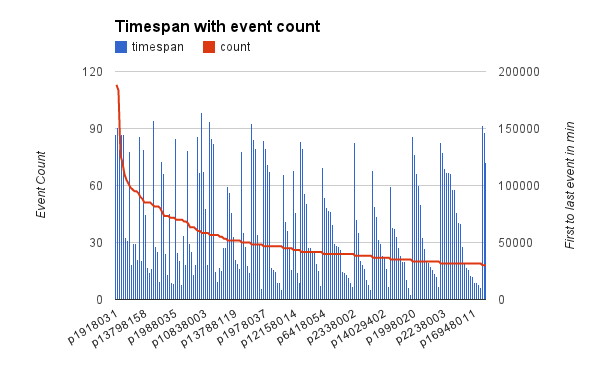
\includegraphics[width=5in]{image/item-timespan-event-count.png}
        \centering
        \caption[Count of sessions per user mapped with count of user with give
        session amount]{TODOsome awesome text}
    \end{figure}

    \begin{figure}[H]
        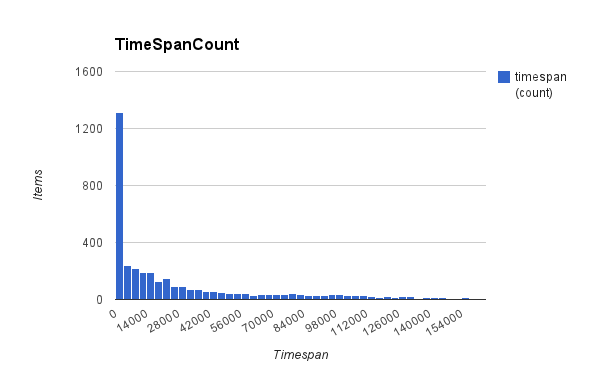
\includegraphics[width=5in]{image/time-span-count.png}
        \centering
        \caption[Count of sessions per user mapped with count of user with give
        session amount]{TODOsome awesome text}
    \end{figure}



    TODO: STRUCTURExfdgdsagCFG

        Blobs of smaller bubbles with eventid
        Blobs for eventcount on stores with items items from stores (populate "storename" for "itemevents")
        Show occurence of event after other event?
        User stats: items, likes, intented purchased, events, session avg, max event, fequency
        Find prices for stores: prize ranges
        User

     Next Monday:
        How to convert
        is the values independent

    is viewing a item (with the possible, albeit unknown intent of consuming) really the same class of problems as actually consuming a item, and how does amount of looking map to amount of consumption?

    transforming implicit feedback into explicit

\subsection{Session Findings}
    Init Hypothesis:
    Two users with similar session habits and similar product accessing pattern
    have a stronger correlation to one-another than two users with just similar
    product interests.


    'product\_purchase\_intended' (user pushed to the product web store) shows a
    wider specter of information about the product, including additional colors,
    images and colors.  For some it might be natural to explore the item there
    before "wanting" it. Making both

    "product\_purchase\_intended" $\Rightarrow$ "product\_wanted"

    and

    "product\_purchase\_intended" $\notimplies$ "product\_wanted"

    produce valuable information.

    Must make different rules for the different stores:
    "Bik Bok", "Cubus", "Gina Trik", "H\&M", "Bianco" has a broad specter of extra
    functions inside the web store, whereas others might not, only shows the
    product and a add to chart button.  This might divide the use pattern of the
    users into a:

    "product\_detail\_clicked" $\Rightarrow$ "product\_purchase\_intended" $\Rightarrow$ "product\_wanted"

    "product\_detail\_clicked" $\Rightarrow$ "product\_purchase\_intended" $\notimplies$ "product\_wanted",

    and

    "product\_detail\_clicked" $\Rightarrow$ "product\_wanted"

    based on the store accessed.

    Use this to make a "rule set" with a probability.
    Then again use this to recommend items for the users with that given
    probability.

    Find a "most popular session"-pattern
    Find a "most likely to come after"-pattern

    Session issues:
    Once in a blue moon a user will do a "product action" (purchase,want,details)
    without having a previous frontstore-access event. Which leads to unknown
    store-id of the item.

    Issue is most probably from missing user-id in collection\_viewed, and a user
    checks out an item from there. It is not possible to be 100\% sure which user
    access the item from the collection\_viewed event, so this event is therefor
    not integrated into the session-stack.
